\section{Application examples}
\label{sec:applications}
The \textit{EnsembleModel} capability has been largely used in the past year, since the increase interest in
integrated analysis involving different physics with a blend of surrogate models.
%In this section a application examples are reported in order to testify and show the potential of this capability.
In this section an application example is reported in order to testify and show the potential of this capability.
\section{Pump Controller Model}
\label{sec:pumpControllerModel}
\begin{figure}
    \centering
    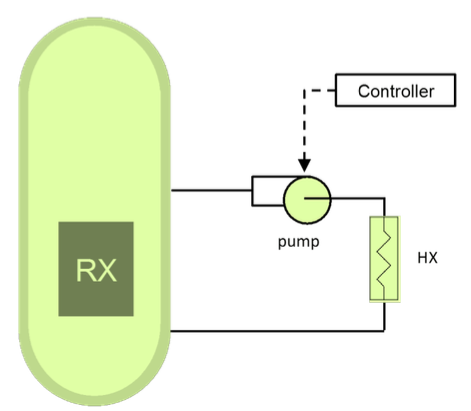
\includegraphics[scale=0.6]{App1_schem_controller.png}
    \caption{Pump controller model scheme}
    \label{fig:ensembleModelApp1Controller}
\end{figure}

\begin{figure}
    \centering
    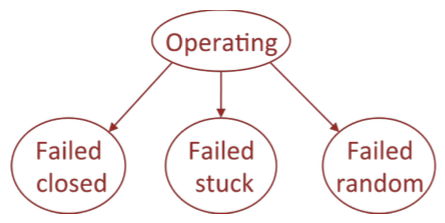
\includegraphics[scale=0.6]{App1_schem_markov.png}
    \caption{Continuos time Markov model for the pump controller}
    \label{fig:ensembleModelAppMarkov}
\end{figure}
\begin{figure}
    \centering
    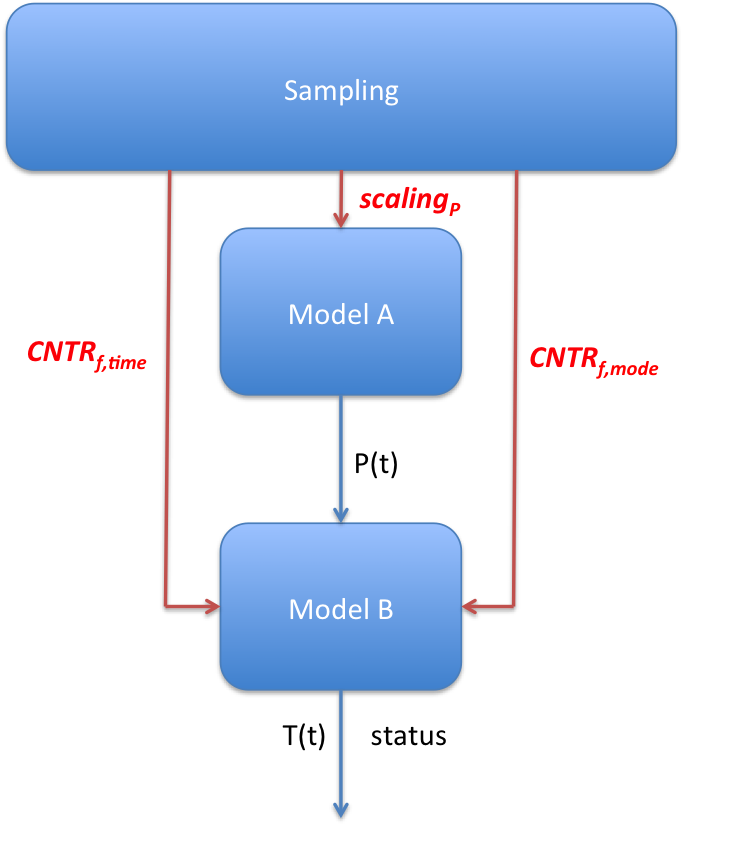
\includegraphics[scale=0.6]{App1_sampling.png}
    \caption{Ensemble Model scheme for PWR controller example}
    \label{fig:ensembleModelApp1sampling}
\end{figure}
The first example here reported is a simplified analysis performed connecting two models in an \textit{EnsembleModel} 
configuration:
\begin{itemize}
  \item A pump controller model (\textbf{Model B}) for a hypothetical simplified PWR model (see Fig. ~\ref{fig:ensembleModelApp1Controller}) has
          been used. It consists of the following components:
          \begin{itemize}
             \item Reactor core (RX)
             \item Motor operated pump
             \item Pump digital controller
             \item Heat exchanger (HX)
          \end{itemize}
          This system is responsible to remove the decay heat generated from the core (RX) in order to avoid damage of the core itself. While we assumed that both 
          the HS and the pump are perfectly reliable components (i.e., no failure can be introduced), using [Ref] as a references, the digital pump controller reliability 
          model has been performed using a continuous time Markov Chain formulation.
          In more detail, the controller has been modeled using 4 states (Fig. ~\ref{fig:ensembleModelAppMarkov}):
          \begin{itemize}    
            \item Operating: controller operating as designed     
            \item Failed closed: controller failed by sending close signal to pump (i.e., pump not running)
            \item Failed stuck: controller failed by sending oldest valid signal to pump  
            \item Failed random: controller failed by sending close signal to pump  
          \end{itemize} 
          In order to perform such analysis the model has been coded as a RAVEN external model
          which determine the temporal profile of core temperature give the two stochastic parameters:
          \begin{itemize}   
            \item Pump controller failure time ($CNTR_{f,time}$)
            \item Pump controller failure mode ($CNTR_{f,mode}$)
          \end{itemize} 
          The dynamic of the hypothetical system has been modeled using basic mass and energy
          conservation laws so no effective engineering conclusions can be gathered by this example.
   \item A power history generator model (\textbf{Model A}) has been used. It employs of the following simple
           equation:    
           \\$𝑃𝑜𝑤𝑒𝑟(𝑡) = 1,500 ∗ 𝑠𝑐𝑎𝑙𝑖𝑛𝑔_{𝑃} ∗ exp(−𝑡)$  
           \\The power multiplier ($scaling_{P}$) is an additional stochastic parameter in this example analysis (Uniform between 0.5 and 1.2).
\end{itemize}
\begin{figure}
    \centering
    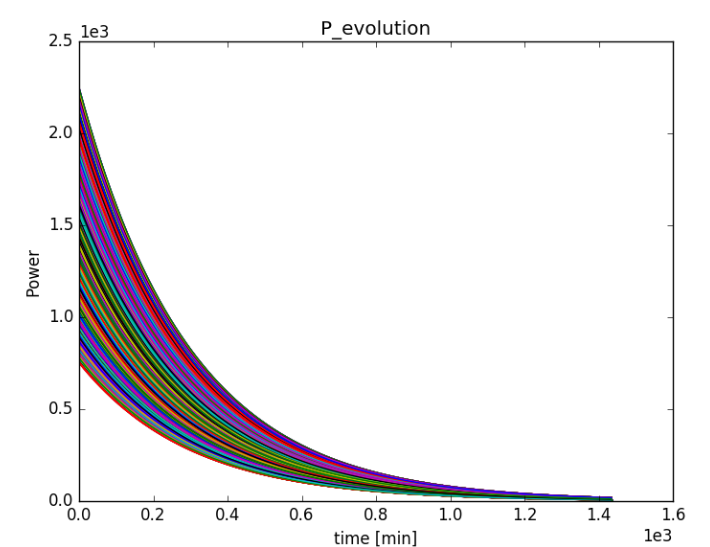
\includegraphics[scale=0.6]{App1_P_evolution.png}
    \caption{Plot of the 1500 histories (Power - Model B) generated by RAVEN}
    \label{fig:ensembleModelApp1Power}
\end{figure}
\begin{figure}
    \centering
    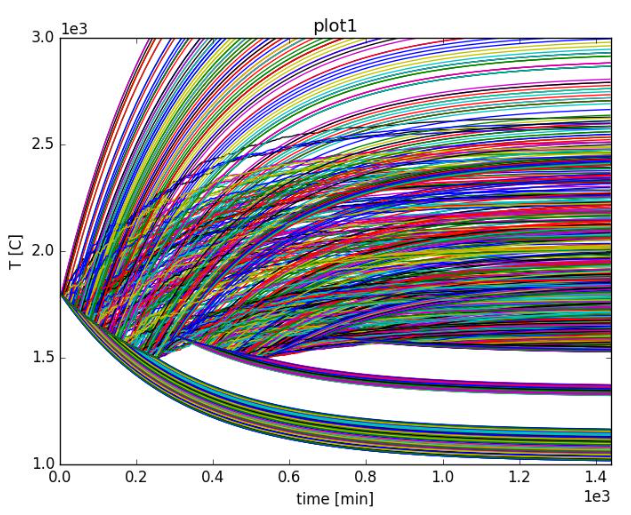
\includegraphics[scale=0.6]{App1_T_evolution.png}
    \caption{Plot of the 1500 histories (Temperature – Model A) generated by RAVEN}
    \label{fig:ensembleModelApp1Temperature}
\end{figure}
The EnsembleModel data flow is shown in Figure ~\ref{fig:ensembleModelApp1sampling}. The Model A generates a Power history (time-dependent) that is passed into the Model B that employs the 
balance analysis. Even if the presented example is quite simplified, it shows the potential of this added capability.
By using RAVEN we sampled the three stochastic parameters using a Monte-Carlo algorithm and generated 1500 simulations as shown in Figures ~\ref{fig:ensembleModelApp1Power} and ~\ref{fig:ensembleModelApp1Temperature}. Note in Figure  ~\ref{fig:ensembleModelApp1Temperature} (i.e., Model B) that in some cases elevated temperatures are recorded due to the potential failures of the pump in the system.
\begin{figure}
    \centering
    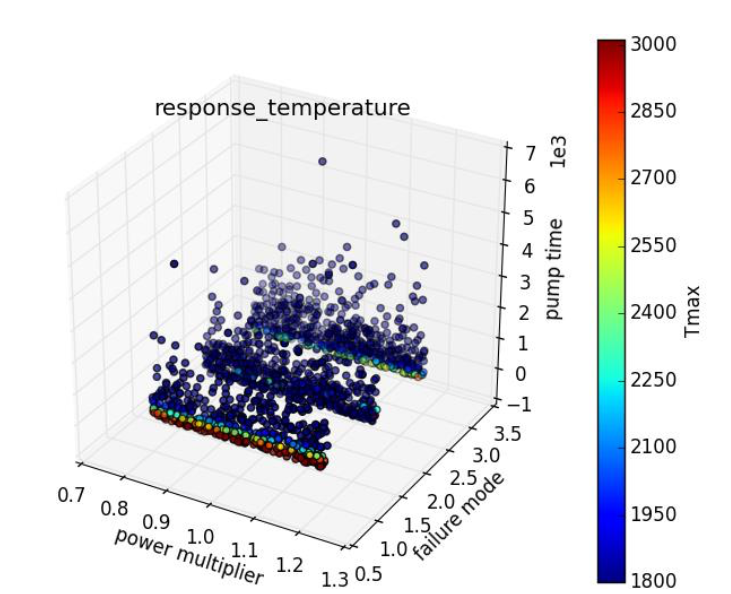
\includegraphics[scale=0.6]{App1_Response_temperature.png}
    \caption{Input space partitioning with respect to maximum temperature in the system}
    \label{fig:ensembleModelApp1RespTemp}
\end{figure}
\begin{figure}
    \centering
    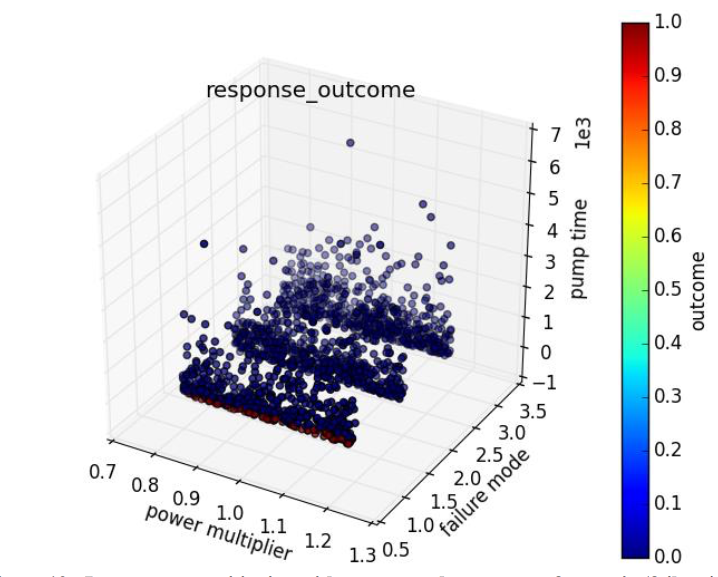
\includegraphics[scale=0.6]{App1_Response_outcomes.png}
    \caption{Input space partitioning with respect to the outcome of scenario (failure/success)}
    \label{fig:ensembleModelApp1RespOutcome}
\end{figure}

In Figures ~\ref{fig:ensembleModelApp1RespTemp}  and ~\ref{fig:ensembleModelApp1RespOutcome}  it can be seen as most of the failures happened in failure mode 1 (i.e. controller failed by sending close signal to pump (i.e., pump not running).
This simple example testifies how RAVEN can share 1-Dimensional Figure of Merits, abstracting the concept of ``input realization'' from scalars (e.g. uncertainty on thermal conductivity) to vectors (e.g. power histories).